\documentclass[landscape,a2paper,fontscale=0.833]{baposter}
\usepackage[utf8]{inputenc}
\graphicspath{ {./images/} }
\usepackage{graphicx}
\usepackage{amsmath}
\usepackage{amsthm}
\usepackage{amssymb}
\usepackage{booktabs}
\usepackage{enumitem}
\usepackage[font=small,labelfont=bf]{caption}
\usepackage{color}
\usepackage{xcolor}
\usepackage{dirtytalk}
\UseRawInputEncoding
\usepackage{caption}
\usepackage{subcaption}
\usepackage{mathtools}
\usepackage[thinc]{esdiff}
\usepackage{multicol}
\usepackage{tocbibind}
\usepackage{parskip}
\usepackage[ruled,vlined]{algorithm2e}
\usepackage{tikz}
\usetikzlibrary{shapes,arrows}
\newtheorem{theorem}{Theorem}
\newtheorem{definition}{Definition}


\begin{document}

\begin{poster}
{
colspacing=1em,
bgColorOne = lime,
bgColorTwo = teal,
borderColor = black,
headerColorOne = yellow,
textborder = roundedsmall,
headerborder = closed,
headerColorOne=black,
headerFontColor=white,
boxColorOne=white,
headerheight=0.1\textheight,
headershape = smallrounded,
headerfont=\Large\bf\textsc,
linewidth=2pt
}

{\bf\textsc{Classification Decision Trees}\vspace{0.5em}} 
{\textsc{Pattanin (Mill) Luangamornlert supervised by Peter Craig and Louis Aslett \hspace{12pt} Durham University}}







\headerbox{What are Decision Trees}{name=intro,column=0,row=0}{
We have a learning set $\{x_i, y_i\}$ and we aim to predict $\hat{y}_i$ given a new datapoint $x_i$. To do this with non-parametric data we use Decision Tree Algorithms which are a method of supervised Machine Learning.
Invented in 1984 \cite{BreimanDT}, 
CART is the most famous and popular method for Decision Trees and relies on checking impurities in the splitting of data in feature selection.
\medskip\\
For a dataset, we aim to split the data $\{x_{i}, y_{i}\}_{i=1}^{n}$ into $R_m$ regions, $m = [1, \dots, M]$.\\
For each split, we calculate a metric from the choice below to decide where to split the data at each partition.
\vspace{1em}
\begin{center}
    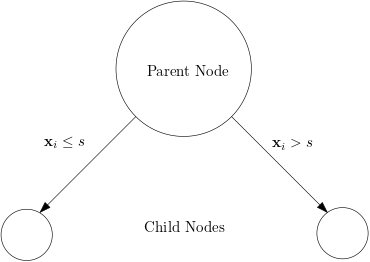
\includegraphics[width=0.5\textwidth]{ipefile/simpledecisionsplit.png}
    \label{fig:dt1}
    \captionof{figure}{Decision Trees split data depending on which side of the cut they are on}
\end{center}

}

\headerbox{Classification Splitting Metrics}{name=metrics,column=0,below=intro}{
To choose where to split, we calculate values at each split. These are called metrics and we recursively calculate these values for each branch to find the optimal value.
Each metric tries to minimize the error when we split the data into two groups. Some of the Classification Metrics which have been used include:
\vspace{0.3em}
\begin{itemize}
    \item Chi-Squared ($\chi^2$) testing for significance of variables
    \[ \chi^{2} = \sum_{i = 1}^{n} \frac{\sqrt{(y_{i} - E(y_{i}))^2}}{E(y_{i})} \]
    We select the splitting point to be the point with the highest value and continue until no significant $\chi^2$ value can be found.
    This is used in the CHAID algorithm by Kass (1980)
    
    \item Information Gain 
    \[  I_G(T,a) = -\sum_{i=1}^{n} p_i \log p_i 
    + \sum_{i=1}^{n} P(i \mid a) \log_2 P(i \mid a) \]
    With probabilities $p_i$, and $P(i \mid a)$ the proportion of the group that was split into one child node $a$ from the parent node.
    This chooses the split which results in us getting the largest increase in information by that split. 
    Used by Quinlan (1986) for ID3, C4.5 etc.
    
    \item Twoing Rule for grouping the whole dataset into two groups $P_L$ and $P_R$
    \[  I_G (p) = \frac{P_L P_R}{4} \left[ \sum_{i=1}^{N} \left| p_{i,L} - p_{i,R} \right| \right]^2 \]
    Where $p_{i,L}$ and $p_{i,R}$ is the probabilities that $p_i$ is grouped into the left or right nodes
    
    \item CART uses \textbf{Gini Impurity} in selecting features.\\
    Gini Impurity is defined as follows:
    \begin{equation}
        I_G (p) = I_G (p_1, \dots, p_M) = \sum_{i=1}^{M} p_i(1-p_i)
    \end{equation}
    With $m = 1,\dots,M$ classes and probabilities $p_i$ with $\sum_{i=1}^{M} p(i) = 1$.\\
    From here we apply this equation to all variables and select the one which provides the highest impurity, i.e. $\max$ $I_G (p)$, as the splitting point.
\end{itemize}
}

\headerbox{References}{name=references,column=1,above=bottom}{

\renewcommand{\section}[2]{\vskip 0.05em} % Get rid of the default "References" section title
\small{ % Reduce the font size in this block
\bibliographystyle{unsrt}
\bibliography{reference} % Use sample.bib as the bibliography file
}}





\headerbox{CART Algorithm}{name=cart,column=1,row=0}{
\begin{enumerate}
\item Use recursive splitting at all points into regions $R_1, R_2$ such that for a splitting value $s$, we have that for each value $x_i$, $i \in [1, \dots, n]$:
\begin{enumerate}
    \item $R_1 = x_i \leq s$
    \item $R_2 = x_i > s$
\end{enumerate}
and classify each prediction in region based on the mean/modal value in each region
     
\item Calculate the metric value for each region
     
\item Compare metric values to find the most optimal splitting point
     
\item Repeat until stopping criterion met
\end{enumerate}
}


\headerbox{Pruning}{name=prune, column=1,row=1,below=cart}{
To achieve interpretability, we would prefer smaller trees. However, growing small trees would hide useful splits hidden under weak splits. Therefore a more optimal approach would be to grow the tree and then cut back to a more optimal size.\\
The idea of pruning is to minimise the cost-complexity criterion $C_{\alpha} (T)$:
\begin{equation} \label{eq:prune}
    C_{\alpha} (T) = R(T) + \alpha \left|T\right|
\end{equation}
Where $R(T)$ is the learning error, $\left|T\right|$ the number of terminal nodes in tree $T$, and $\alpha$ the regularization parameter. We find that $\alpha$ can be obtained from:
\[ \alpha = \frac{R(t)-R(T_t)}{|T_t| - 1} \]
And we are able to select the smallest value of $\alpha$ which minimizes equation~\ref{eq:prune}. Note that if $\alpha = 0$, we return an unpruned tree.
\medskip\\
The algorithm for this is as such:
    \begin{enumerate}
        \item Initialization - Let $T^1$ be the tree obtained with $\alpha^1 = 0$ by minimizing $R(T)$
    
        \item Select $t \in T^1$ which minimizes
        \[ g_1 (t) = \frac{R(t)-R(T_t^1)}{|T_t^1| - 1} \]
    
        \item Let $t_1$ be this node and let $\alpha^2 = g_1 (t_1)$ which results in $T^2 = T^1 - T_{t_1}^1$
    
        \item Repeat the process $i$ times until at cost $k$
    \end{enumerate}
    After pruning, we have found an optimal tree, up to cost, which provides the highest accuracy score.
}

\headerbox{Note on Regression}{name=reg,column=1,row=2,below=prune}{
Regression CART uses a very similar method as classification but because there is no natural grouping of predictors, an alternative method is used.
Suppose we have a space $R$ and we have $M$ partitions, we first partition the space into $M$ regions $R_1, \dots, R_M$.\\
 To construct the regions, we try to find regions which minimize \textbf{RSS - The Residual Sum of Squares}, where we have $\hat{y}_{R_m}$ as the mean response for each region:
 \begin{equation}
    RSS = \sum_{m=1}^{M} \sum_{i \in R_m} (y_i - \hat{y}_{R_m})^2
 \end{equation}
 From here we apply this equation to all variables and select the one which provides the smallest error, i.e. $\min$ RSS, as the splitting point.
 This equation is:
 \begin{equation}
    \min \sum_{x_i \in R_1} (y_i - \hat{y}_{R_1})^2  +  \sum_{x_i \in R_2} (y_i - \hat{y}_{R_2})^2
 \end{equation}

}

\headerbox{Example of a Classification Decision Tree using CART}{name=example,column=2,span=2,row=0}{
\begin{multicols}{2}
\begin{center}
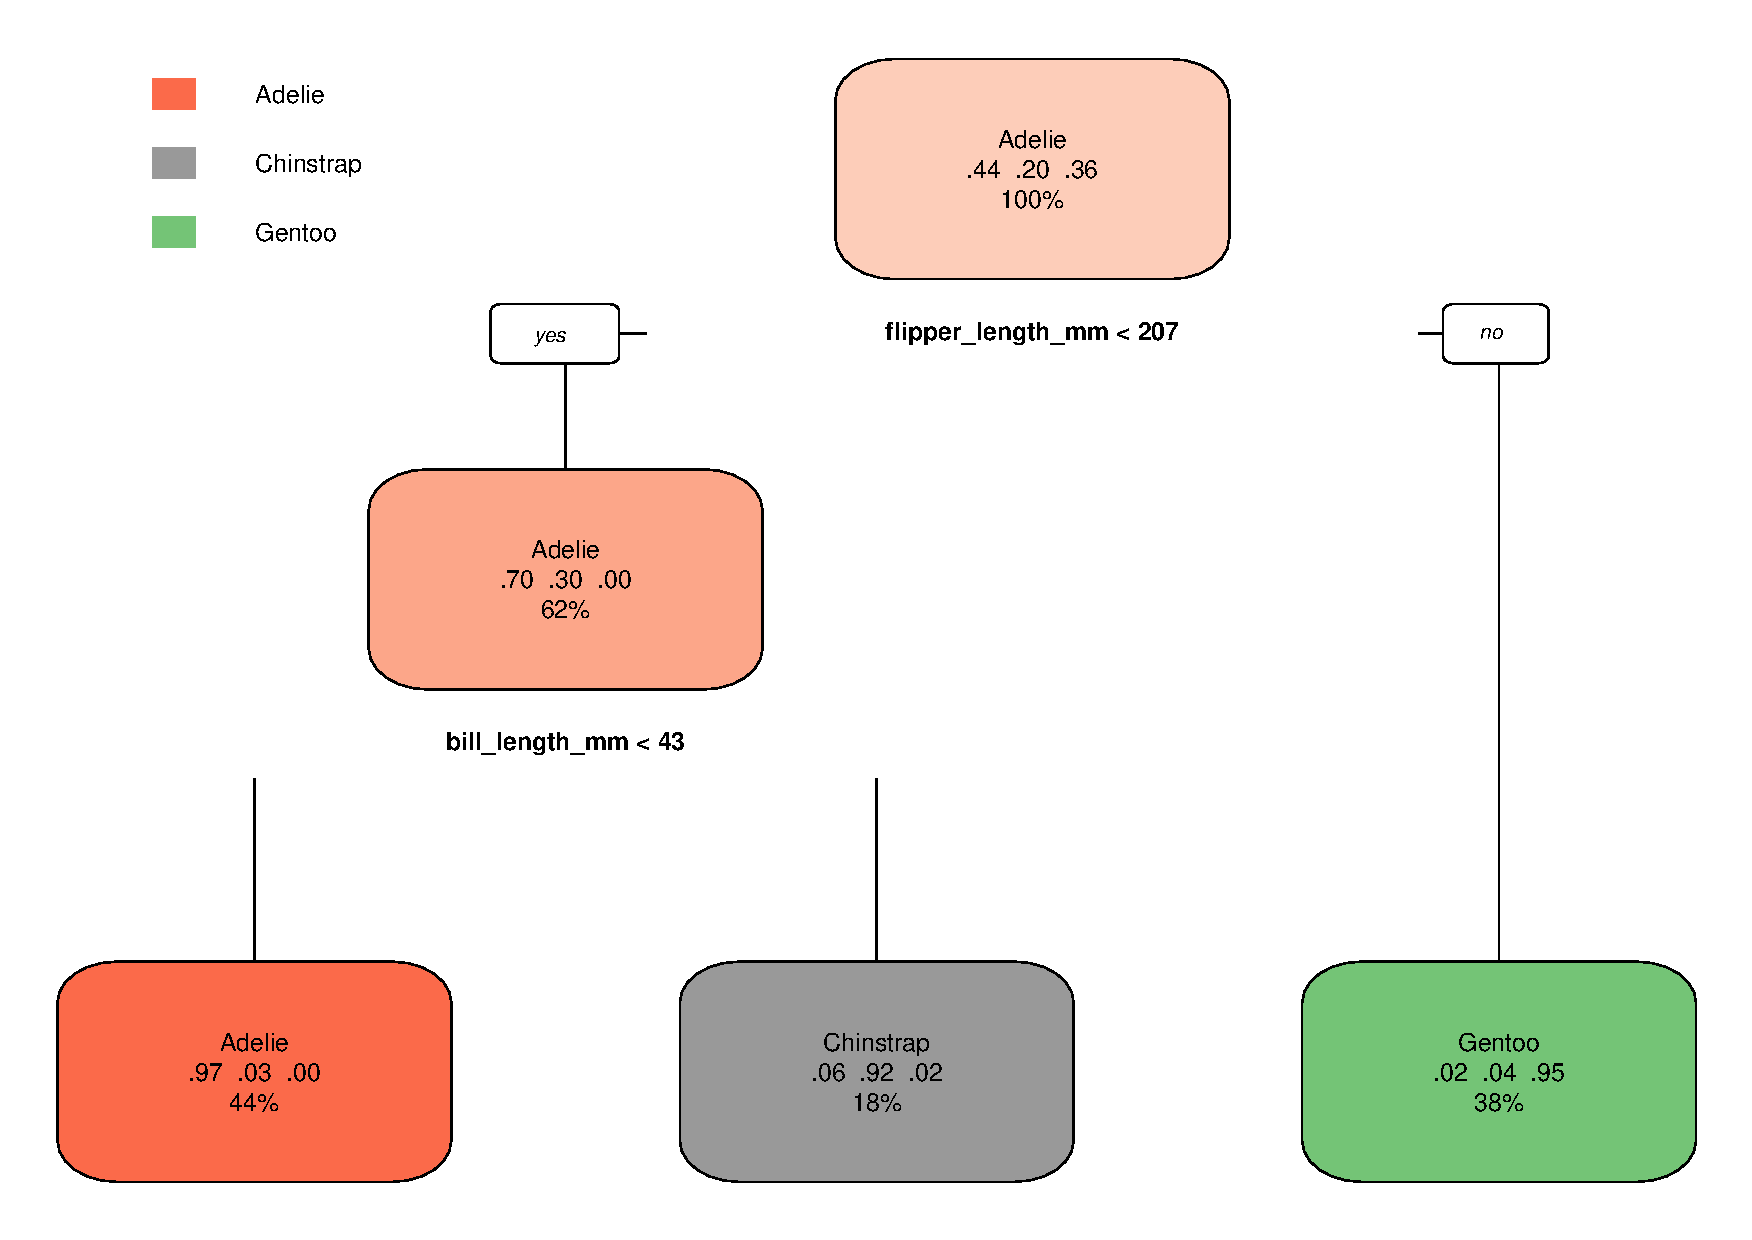
\includegraphics[width=0.8\linewidth]{presentation/Penguintree.pdf}
\label{fig:penguins}
\captionof{figure}{An Example of a Decision Tree using the \texttt{Penguins} dataset (Horst)}
\end{center}


\begin{center}
    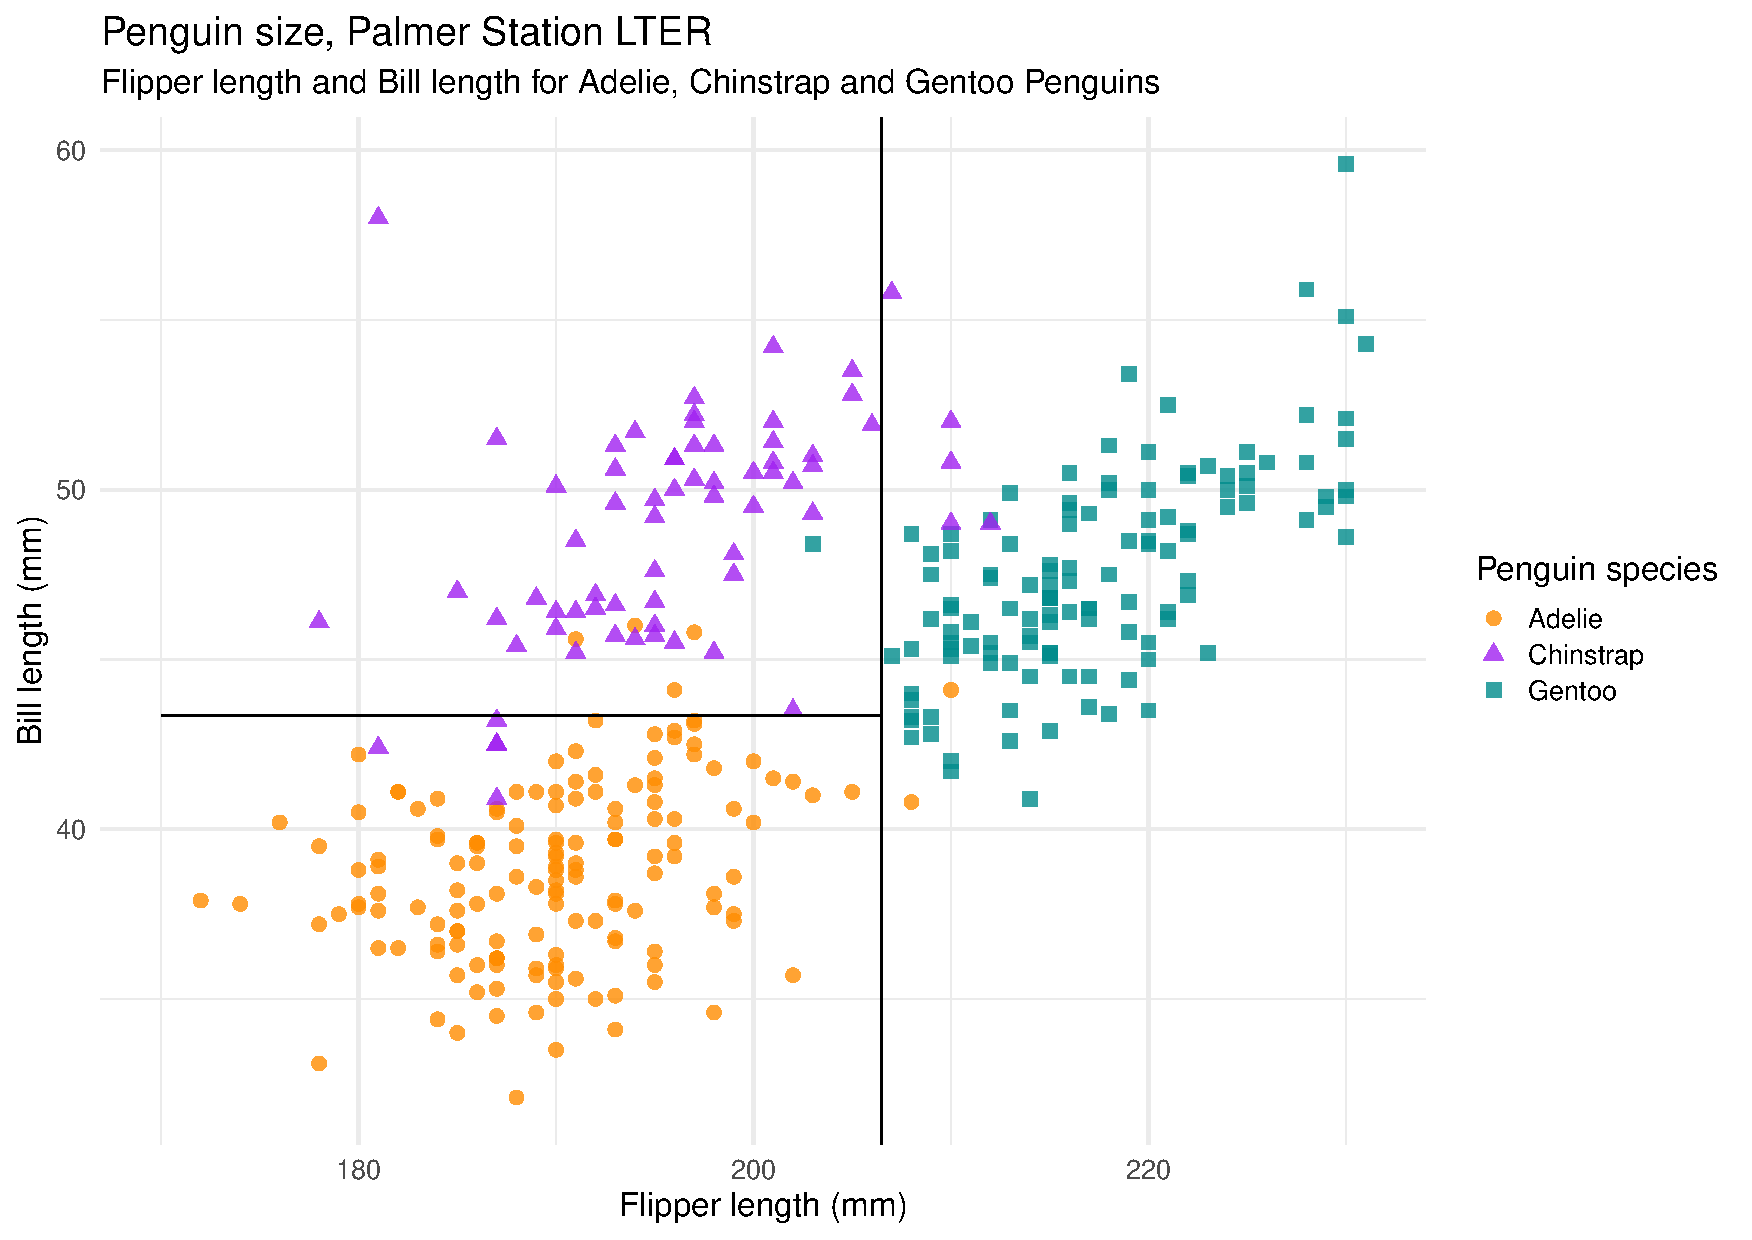
\includegraphics[width=0.8\linewidth]{presentation/plotpen2.pdf}
    \label{fog:penplot}
    \captionof{figure}{Plot of Penguins data with our Decision Tree Splits}
\end{center}
\end{multicols}
We use the \texttt{penguins} dataset to form a decision tree. 
This can be displayed on a plot to show where each decision split is made, with the first split (The top branch on the tree) corresponding to the split along the line at \texttt{x = 206.5} and the second split (The second branch on the left child node) corresponding to the split along the line at \texttt{y = 43.35} up to the first split.
This forms the three regions that we have created in the decision tree.
}

\headerbox{Example of Pruned Tree}{name=example2,column=2,below=example}{
Here, we use the \texttt{Pima} dataset to show how pruning affects our decision tree. 
\begin{center}
    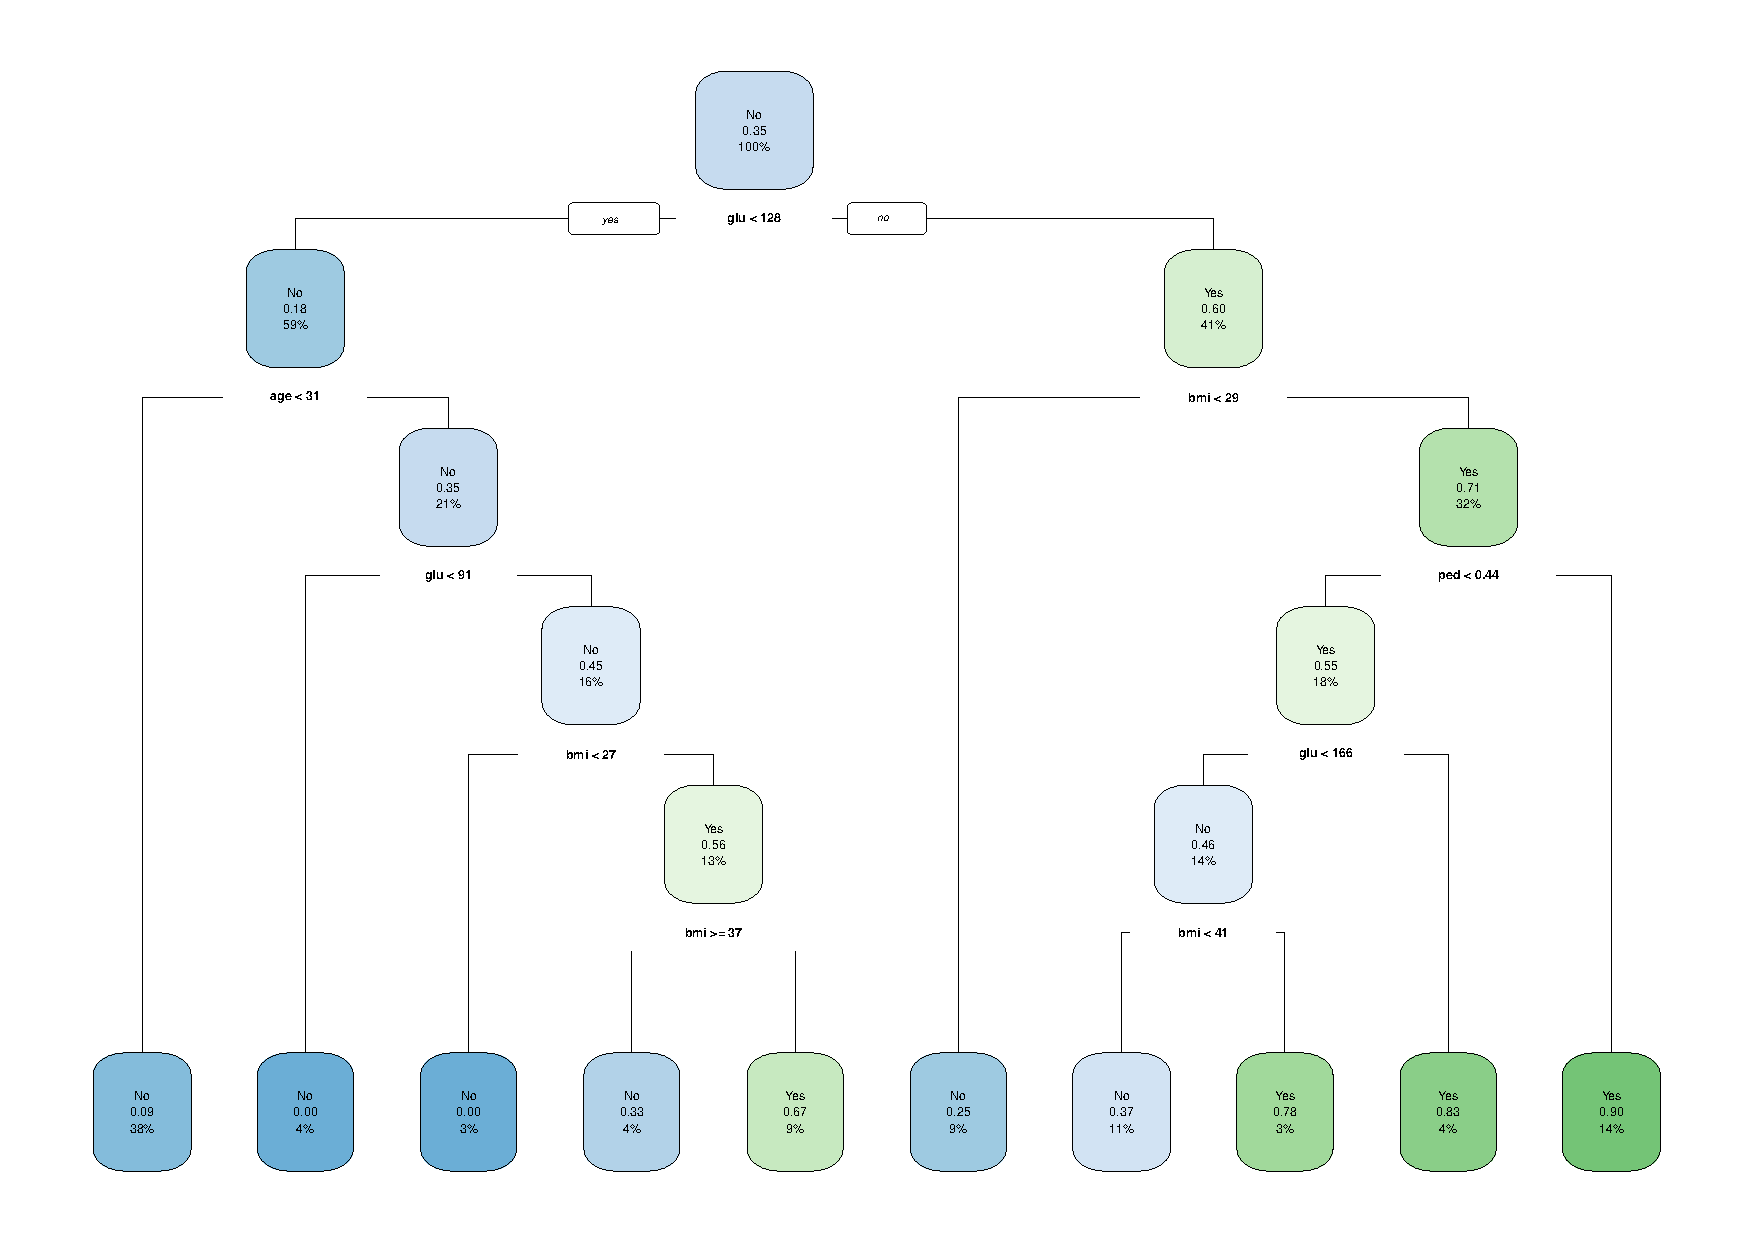
\includegraphics[width=0.75\linewidth]{presentation/pimatrain.pdf}
    \label{fig:pima1}
    \captionof{figure}{Full Grown Pima Decision Tree}
\end{center}

\begin{center}
    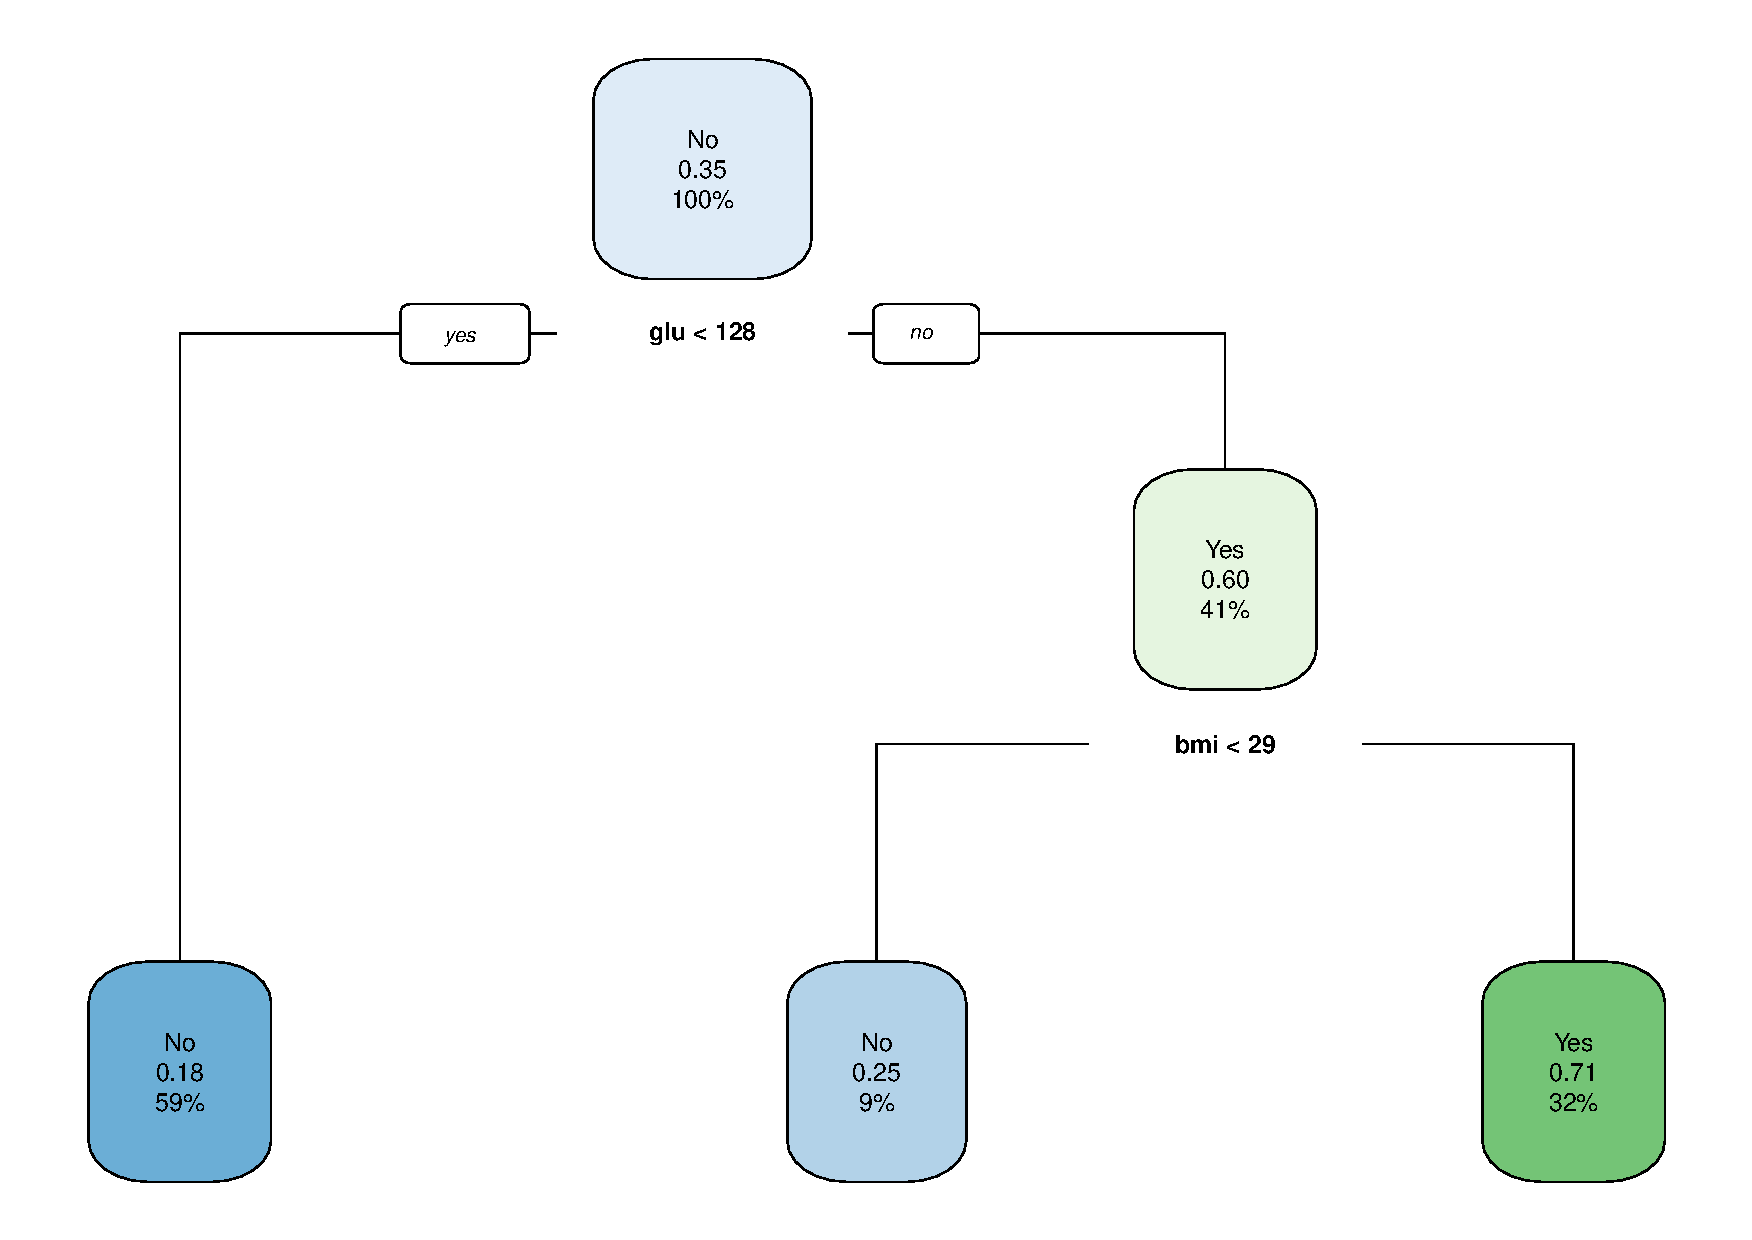
\includegraphics[width=0.7\linewidth]{presentation/pimaprune.pdf}
    \label{fig:pima2}
    \captionof{figure}{Pruned Pima Decision Tree}
\end{center}


}

\headerbox{Testing Pruning Performance}{name=prune,column=3,below=example}{
We use the \textbf{Receiver Operating Characteristic Curve} (ROC) to show how well a classification model, e.g. the Pima  predicts data. 
An ideal model would have a curve with an area, called the AUC, close to 1, while a model whose ROC line goes below the dotted line is deemed worse than tossing a biased coin.
\vspace{0.3em}
\begin{center}
    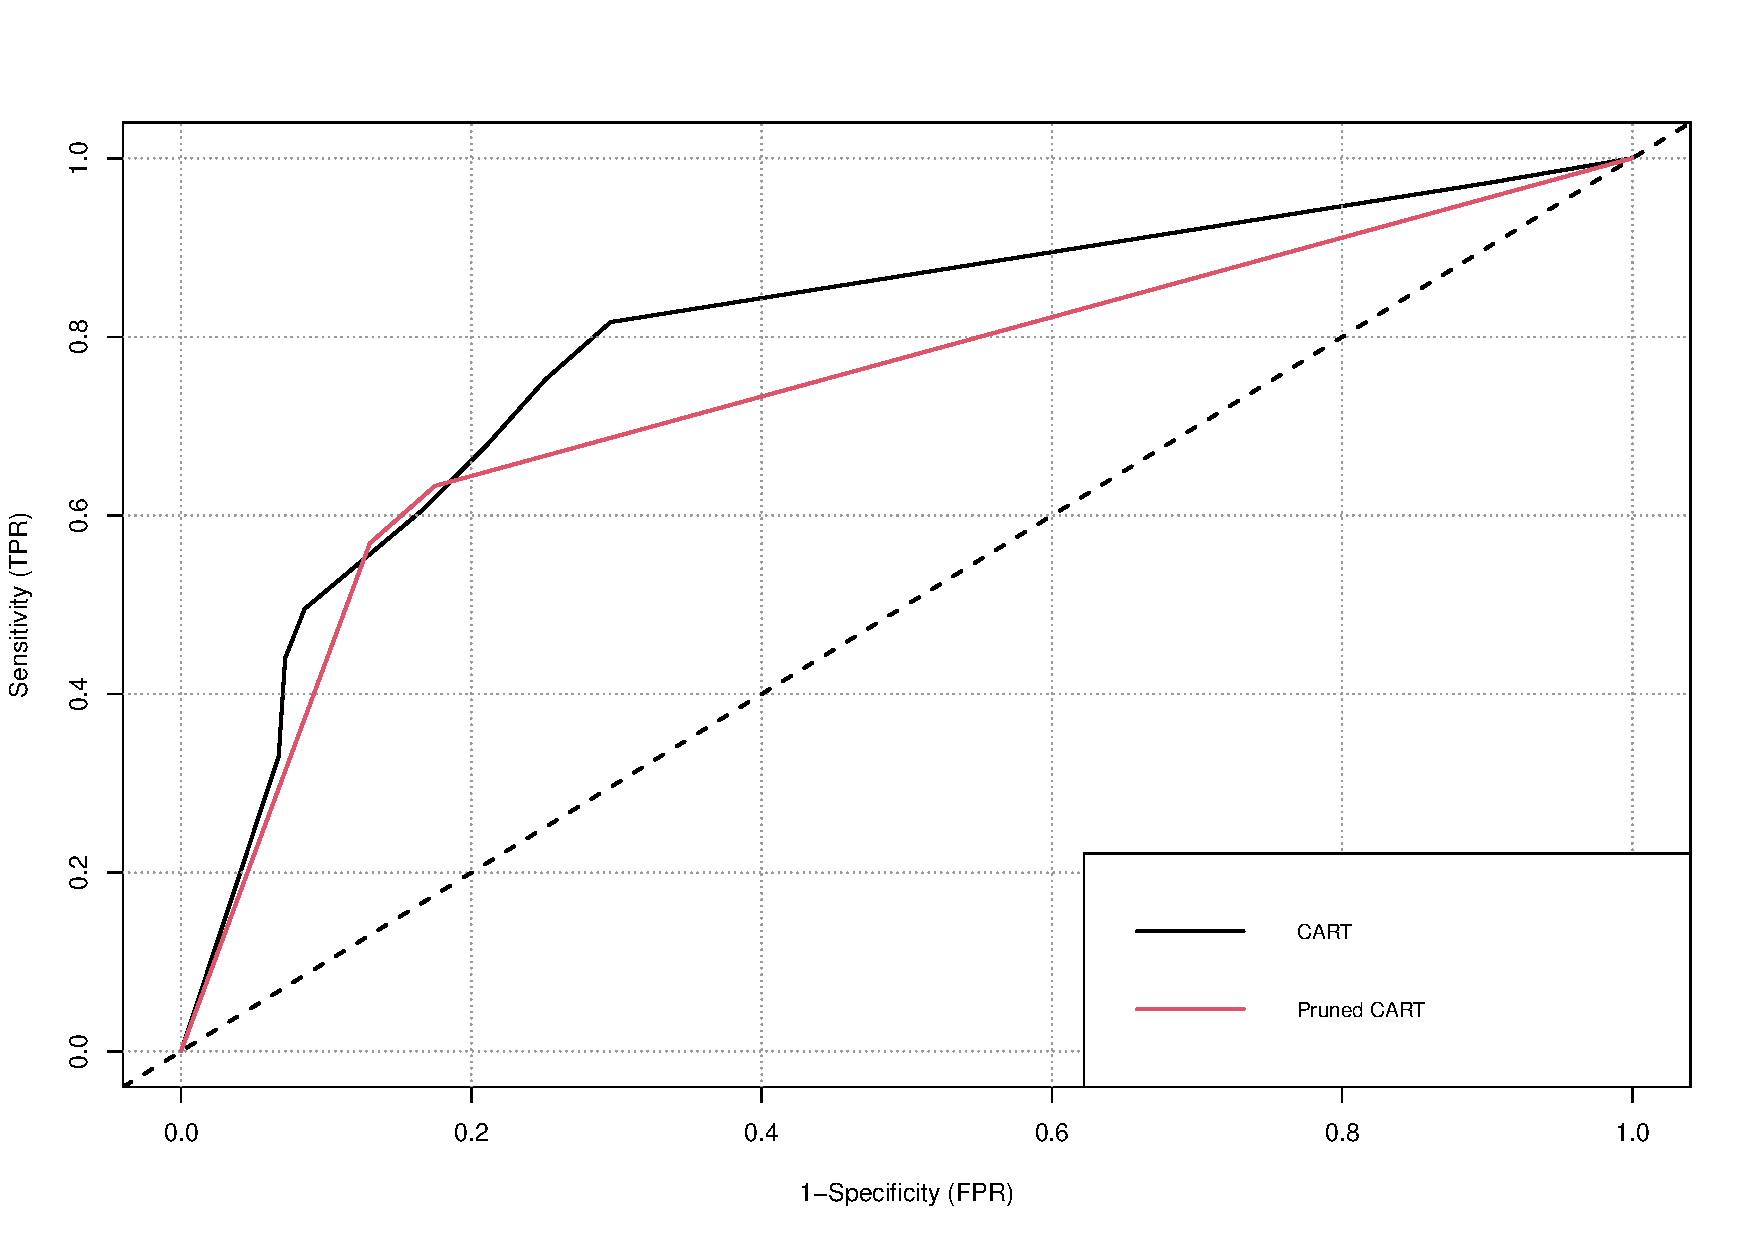
\includegraphics[width=0.8\linewidth]{presentation/pimaroc.pdf}
    \label{fig:pimaroc}
    \captionof{figure}{ROC Curves to show accuracy of Decision Trees}
\end{center}
\vspace{1em}
In this case, this model gives the following ROC results:
\medskip
\begin{center}
    \begin{tabular}{|c|c|c|c|}
        \cline{2-4}
        \multicolumn{1}{c|}{} & Estimate AUC & 2.5\% CI & 97.5\% CI \\
        \hline
        Normal ROC & 0.7952 & 0.7402 & 0.8503 \\
        \hline
        Pruned ROC & 0.7376 & 0.6777 & 0.7976 \\
        \hline
    \end{tabular}
\end{center}
\medskip
We have that the pruned tree performs slightly worse than the full tree. However, it is much simpler being only a \textit{two-step tree} instead of a \textit{five-step tree} and may be preferred in most scenarios unless very high accuracy is needed.
\vspace{1em}
}

\headerbox{Improving Decision Trees}{name=improve,column=2,span=2,below=example2}{
While Decision Trees are a nice way to predict data, they suffer from the heuristically greedy nature of the top-down approach of the algorithm.
Many methods have been invented to try to improve this, and has led to two approaches:
\begin{enumerate}
    \item \textbf{Ensemble Methods} - These methods include bagging, random forests and boosting. They attempt to aggregate multiple trees which have been formed from bootstrapping the learning set to form many \textit{"weak learning"} trees. This can be implemented using \texttt{randomForest} in \texttt{R}.
    
    \item \textbf{Optimization of Algorithm} - This method attempts to change either the metrics involved or the algorithm used to improve the split.
    A modern approach is using the Optimized Trees methods by Bertsimas and Dunn (2017) \cite{oct} which is implemented via the \texttt{Gurobi Optimization} using the \texttt{Interpretable AI} interface in \texttt{Julia} which solves the decision tree in one go as a Mixed-Integer Programming problem.
\end{enumerate}
}

\end{poster}




\end{document}